\begin{center}{\bf ПРИМЕРЫ СЛОЕНИЙ ЛИУВИЛЛЯ ТОПОЛОГИЧЕСКИХ БИЛЛИАРДОВ, ОГРАНИЧЕННЫХ ДУГАМИ СОФОКУСНЫХ КВАДРИК НА ПЛОСКОСТИ МИНКОВСКОГО} \\
{\it E.E. Каргинова } \\
(Москва; {\it karginov13@gmail.com} )
\end{center}
\addcontentsline{toc}{section}{Каргинова Е.E.}



\textbf{Определение~1.}  {\it Плоскостью Минковского называется $\mathbf R^2$ со скалярным произведением $$\langle x,y\rangle=x_1 y_1-x_2 y_2$$.}


Рассмотрим на плоскости Минковского эллипс $\EuScript E$, задаваемый соотношением:
$$\EuScript E \colon \frac{x^2}{a}+\frac{y^2}{b}=1$$
Здесь $a>b>0$ и $\lambda \in \mathbf{R}$ - вещественные числа. Софокусное семейство квадрик $C_\lambda$ задаётся уравнением
$$C_\lambda \colon \frac{x^2}{a-\lambda}+\frac{y^2}{b+\lambda}=1\eqno (1)$$

В. Драгович  и М. Раднович в работе [2] исследовали биллиард в эллипсе на плоскости Минковского. Для описания топологии слоения Лиувилля ими был применён метод Фоменко-Цишанга. заключающийся в нахождении графа с метками, который является инвариантом интегрируемой системы и полностью определяет топологический тип его слоения Лиувилля. Данный подход подробно изложен в [1].

\textbf{Определение~2.} {\it Простым биллирадом назовём двумерное, связное, плоское, компактное многообразие с кусочно-гладким краем, состоящим из сегментов квадрик семейства (1), попарно пересекающихся под углами, не превышающими $\pi$.}

\textbf{Определение~3.} {\it Топологическим биллиардом называем двумерное ориентируемое многообразие с кусочно-гладкой метрикой Минковского, полученное отождествлением (склейкой) простых биллиардов вдоль некоторых выпуклых или прямолинейных сегментов.}
%Определим отражение на границе простого биллиарда следующим образом: если точка $(x,y)$ лежит на границе области, то вектор $(x,y,v_1,v_2)$ % при отражении от границы переходит в вектор $(x,y,w_1,w_2)$, такой, что:

Данная конструкция была предложена В. В. Ведюшкиной в работе [3].

Определим отражение в топологическом биллиарде следующим образом - при попадании на границу склейки точка продолжает движение по другому листу, а при попадании в угол или ребро, не являющееся ребром склейки, точка продолжает движение так же, как и в случае плоской области.
%\begin{itemize}
%\item $(v_1,v_2)\in l_1, (w_1,w_2) \in l_2$, при этом $l_1$ является биллиардным отражением прямой $l_2$;
%\item $v_1^2+v_2^2=w_1^2+w_2^2$.
%\end{itemize}

%В случае топологического биллиарда отражение на ребрах, не являющихся ребрами склейки, определено аналогично. Если ребро является ребром склейки, то к вышеуказанным условиям добавляется следующее условие:

%\begin{itemize}
%\item точки $(x,y,v_1,v_2)$ и $(x,y,w_1,w_2)$ принадлежат разным простым областям.
%\end{itemize}

При таком отражении сохраняется $\lambda$ - каустика траектории. Имеем два первых интеграла - $\lambda$ и квадрат евклидовой длины вектора скорости $v_E$. Поскольку эти интегралы функционально независимы и находятся в инволюции, простой и топологический биллиарды интегрируемы по Лиувиллю.

Ограничивая систему на поверхность уровня интеграла $v_E$, получим трёхмерное многообразие, называемое изоэнергетичекой поверхностью $Q^3$. В зависимости от изменения $\lambda$ оно расслаивается на двумерные поверхности.


\textbf{Предложение 1.} {\it На рис.\ref{ex} изображены инварианты Фо\-ме\-н\-ко-Ци\-ша\-н\-га изоэнергетических многообразий следующих топологических биллиардов: два склеенных по границе эллипса, два склеенных по выпуклой части границы половины эллипса и две области, полученные пересечением двух эллипсов на плоскости Минковского и координатных осей, склеенные по прямым сегментам границы.}

\begin{figure}[h!]
		\center{ 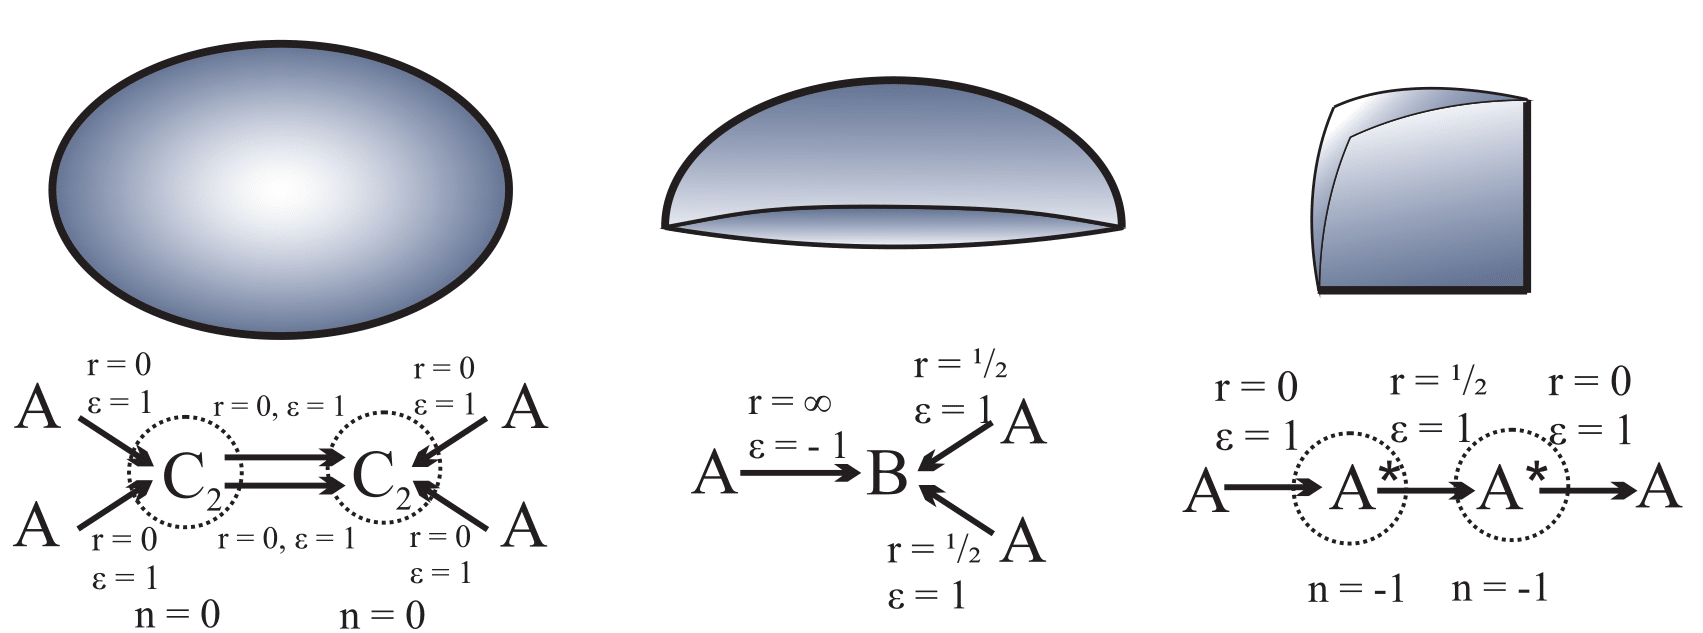
\includegraphics[width=\textwidth]{Karginova_examples2.png}}
		\vspace*{-0.8 cm}
		\caption{Инварианты Фоменко-Цишанга для указанных топологических биллиардов.}
		\label{ex}
	\end{figure}

Исследование выполнено за счёт гранта Российского научного фонда (проект №17-11-01303)

\smallskip \centerline{\bf Литература} \nopagebreak

1. {\it Болсинов А. В., Фоменко А. Т.} Интегрируемые гамильтоновы системы. Геометрия, топология, классификация.  Ижевск НИЦ <<Регулярная и хаотическая динамика>>, 1999. - Т.1


2. {\it Драгович, В., Раднович, М.} Топологические инварианты эллиптических биллиардов и геодезических потоков на эллипсоиде. Фундаментальная и прикладная математика. - 2015. - Т. 20(2), -  С. 51-64.

3. {\it Ведюшкина В.В.} Топологическая классификация биллиардов в локально плоских областях,
ограниченных дугами софокусных квадрик, Матем. сб., 206:10 (2015), 127-176

